%%%%%%%%%%%%%%%%%%%%%%%%%%%%%%%%%%%%%%%%%%%%%%%%%%%%%%%%%
%%             东南大学数电实验报告 LaTeX 模板
%%                SEU-Circuit-Report.cls
%% https://github.com/Teddy-van-Jerry/SEU_Digital_Report
%% ======================================================
%% 版本信息:
%% v1.0 (Nov. 07, 2021)
%% ------------------------------------------------------
%% 模板制作:
%% Teddy van Jerry, (me@teddy-van-jerry.org)
%% * GitHub: https://github.com/Teddy-van-Jerry
%% * Website: https://teddy-van-jerry.org
%% * Blog: https://blog.teddy-van-jerry.org
%% ------------------------------------------------------
%% 使用说明:
%% 1. 编译使用 XeLaTeX 和 Biber
%% 2. 报告基本信息通过修改导言区以 exp 开头的命令
%% 3. 参考文献位于 ref/ref.bib
%% 4. 报告模板依据 MIT License 开源共享
%% ------------------------------------------------------
%% Copyright 2021 (c) Teddy van Jerry
%%
%% Permission is hereby granted, free of charge, to any
%% person obtaining a copy of this software and
%% associated documentation files (the "Software"), to
%% deal in the Software without restriction, including
%% without limitation the rights to use, copy, modify,
%% merge, publish, distribute, sublicense, and/or sell
%% copies of the Software, and to permit persons to whom
%% the Software is furnished to do so, subject to the
%% following conditions:
%%
%% The above copyright notice and this permission notice
%% shall be included in all copies or substantial
%% portions of the Software.
%% 
%% THE SOFTWARE IS PROVIDED "AS IS", WITHOUT WARRANTY OF
%% ANY KIND, EXPRESS OR IMPLIED, INCLUDING BUT NOT
%% LIMITED TO THE WARRANTIES OF MERCHANTABILITY, FITNESS
%% FOR A PARTICULAR PURPOSE AND NONINFRINGEMENT. IN NO
%% EVENT SHALL THE AUTHORS OR COPYRIGHT HOLDERS BE LIABLE
%% FOR ANY CLAIM, DAMAGES OR OTHER LIABILITY, WHETHER IN
%% AN ACTION OF CONTRACT, TORT OR OTHERWISE, ARISING
%% FROM, OUT OF OR IN CONNECTION WITH THE SOFTWARE OR THE
%% USE OR OTHER DEALINGS IN THE SOFTWARE.
%%%%%%%%%%%%%%%%%%%%%%%%%%%%%%%%%%%%%%%%%%%%%%%%%%%%%%%%%%

%% 使用实验报告模板类(字体大小 11pt 约为五号字)
\documentclass[11pt]{SEU-Digital-Report}

%%%%%%%%%%%%%%%%%%%% 报告基本信息 %%%%%%%%%%%%%%%%%%%%
\expno{一} % 实验序号
\expname{数据传送} % 实验名称
\expauthor{薛宇飞 } % 姓名
\expID{04020235} % 学号
\expmates{} % 同组
\expmatesID{} % 学号(同组)
\expmajor{信息工程} % 专业
\explab{金智楼硬件实验室} % 实验室
\expdate{\today} % 实验日期
\expreportdate{\today} % 实验日期
\expgrade{} % 成绩评定
\exptutor{裴文江} % 评阅教师
%%%%%%%%%%%%%%%%%%%%%%%%%%%%%%%%%%%%%%%%%%%%%%%%%%%%
% \usepackage{xeCJK}
\usepackage{threeparttable} %table添加注释
\usepackage{colortbl}
\newcommand{\grayrow}{\rowcolor[rgb]{ .906, .902, .902}}
\usepackage{pgfplots}
\pgfplotsset{compat=1.11}

%% 报告正文
\begin{document}

% 打印封面页
\exptitlepage

\tableofcontents
\newpage

\section{实验目的与内容}       
\begin{enumerate}
    \item 熟悉 8086 指令系统的数据传送指令,进一步掌握传送指令的寻址方式;
    \item 结合实验教材 \cite{book,guide},利用 \texttt{Turbo Debugger (TD)} 调试工具来调试汇编程序。   
\end{enumerate}

\section{实验任务}
实验全部资料及完整代码详见薛宇飞的 \texttt{GitHub} 主页 \cite{mygit}。

\subsection{执行代码段,熟悉 \texttt{TD} 的使用}
程序段如下:
\begin{lstlisting}[language={[x86masm]Assembler},title=code]
    MOV BL,08H
    MOV CL,BL
    MOV AX,03FFH
    MOV BX,AX
    MOV DS:[0020],BX
\end{lstlisting}

实验结果如图 \ref{fig:rlt2}。
\begin{figure}[htbp]
    \centering
    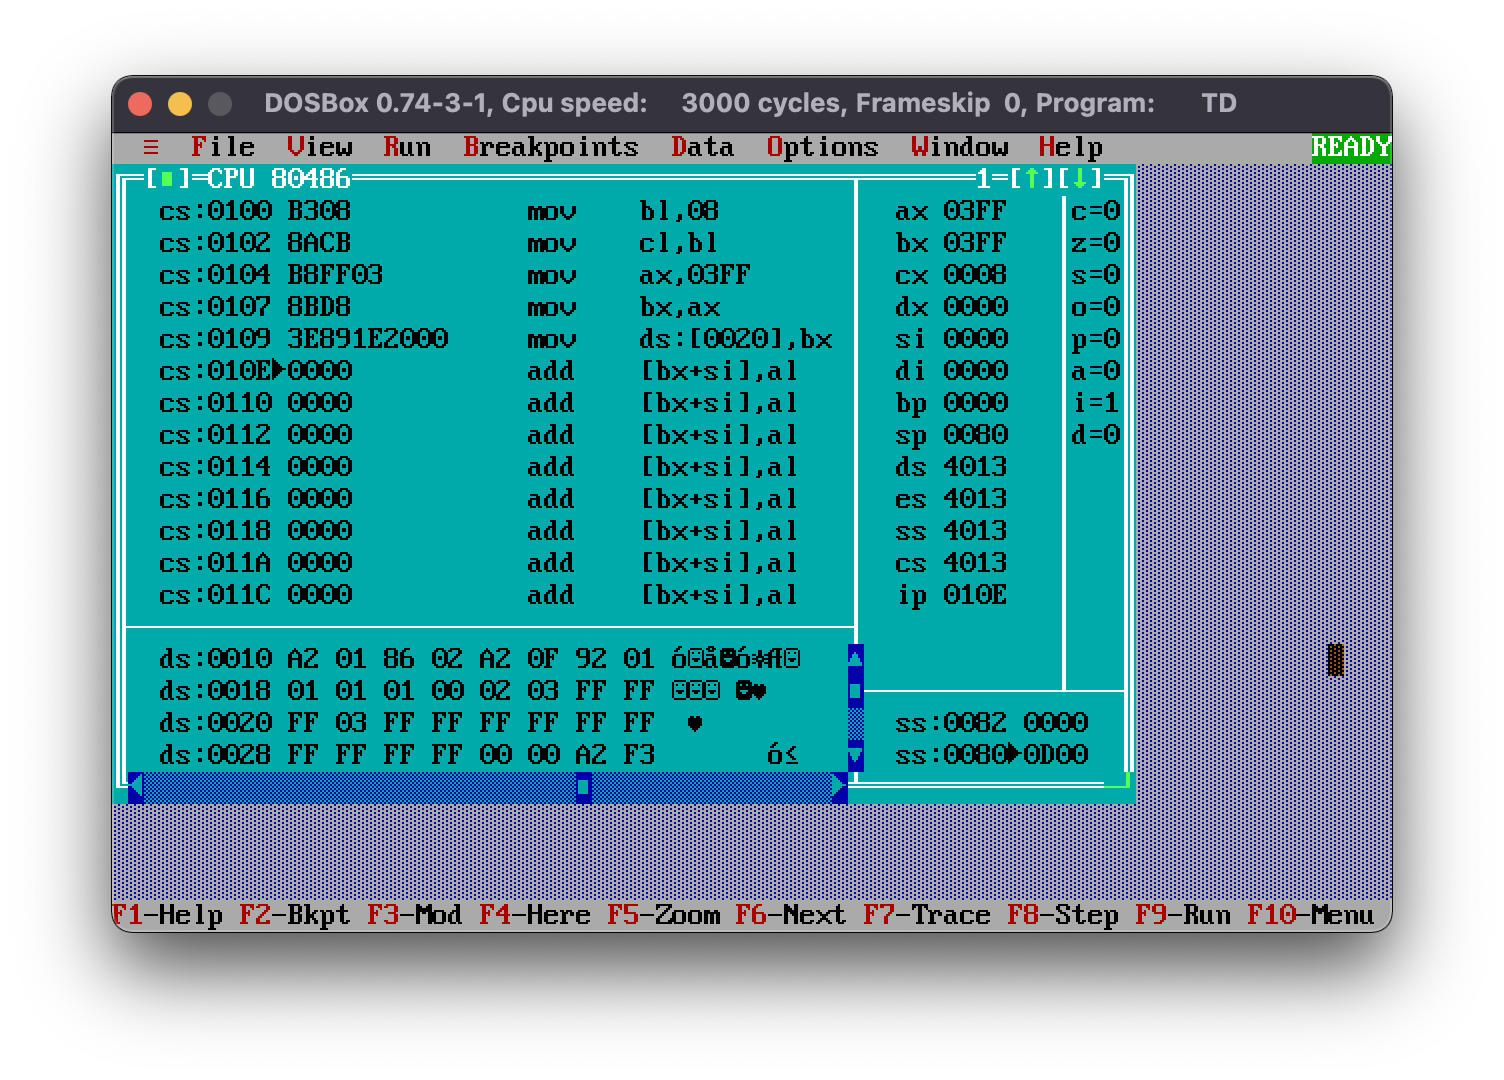
\includegraphics[width=0.7\textwidth]{fig/rlt1.png}
    \caption{实验结果}
    \label{fig:rlt2}
\end{figure}


\subsection{观察不同出栈方式的数据变化}
预备程序段如下:
\begin{lstlisting}[language={[x86masm]Assembler},title=pre-code]
    MOV AX,0102H
    MOV BX,0304H
    MOV CX,0506H
    MOV DX,0708H
    PUSH AX
    PUSH BX
    PUSH CX
    PUSH DX
\end{lstlisting}

第一种出栈方式:
\begin{lstlisting}[language={[x86masm]Assembler},title=way1]
    POP DX
    POP CX
    POP BX
    POP AX
\end{lstlisting}

第二种出栈方式:
\begin{lstlisting}[language={[x86masm]Assembler},title=way2]
    POP AX
    POP BX
    POP CX
    POP DX
\end{lstlisting}

第三种出栈方式:
\begin{lstlisting}[language={[x86masm]Assembler},title=way3]
    POP CX
    POP DX
    POP AX
    POP BX
\end{lstlisting}

实验结果参见表 \ref{tab:rlt2}。
\begin{table}[htbp]
    \centering
    \caption{实验结果表格 \label{tab:rlt2}}
    \bgroup\def\arraystretch{1}
    \setlength{\tabcolsep}{5mm}
        \begin{tabular}{c|c|c|c}
          \toprule
            & \textbf{方式1} & \textbf{方式二} & \textbf{方式三}\\
            \midrule\midrule
            \grayrow \texttt{AX} & 0102 & 0708 & 0304 \\
            \texttt{BX} & 0304 & 0506 & 0102 \\
            \grayrow \texttt{CX} & 0506 & 0304 & 0708 \\
            \texttt{DX} & 0708 & 0102 & 0506 \\
          \bottomrule
        \end{tabular}
    \egroup
\end{table}

\begin{note}{验证要求}{}
    在验证不同的出栈方式之前,需要先执行预备程序段进行初始化。
\end{note}

\subsection{指出并更正题目中的错误}
具体过程详见表 \ref{tab:task3}
\begin{table}[htbp]
    \centering
    \caption{实验任务三\label{tab:task3}}
    \bgroup\def\arraystretch{1}
    \setlength{\tabcolsep}{3mm}
        \begin{tabular}{l|c|c}
          \toprule
            \textbf{错误指令} & \textbf{错误类型} & \textbf{更正(不唯一)}\\
            \midrule\midrule
            \grayrow \texttt{MOV [BX],[SI]} & 目标和源操作数不能同时为寄存器 & \texttt{MOV BX,[SI]}\\
            \texttt{MOV AH,BX} & 源操作数和目标操作数的字长不一致 &  \texttt{MOV AX,BX}\\
            \grayrow \texttt{MOV AX,[SI][DI]} & \texttt{SI,DI}不能同时出现 & \texttt{MOV AX,[BX][DI]} \\
            \texttt{MOV BYTE PTR [BX],2000H} & 源操作数和目标操作数的字长不一致 & \texttt{MOV WORD PTR [BX],2000H} \\
            \grayrow \texttt{MOV CS,AX} & 目标不能是\texttt{CS} & \texttt{MOV BX,AX}\\
            \texttt{MOV DS,2000H} & 立即数不能直接送到段寄存器 & \texttt{MOV BX,2000H}\\
          \bottomrule
        \end{tabular}
    \egroup
\end{table}

\subsection{设置寄存器的内容并验证}
\texttt{BX=0010H, SI=0001H, DS:[0010]=12H, DS:[0011]=34H, DS:[0012]=56H,} 

\texttt{DS:[0013]=78H, DS:[0120]=0ABH, DS:[0121]=0CDH, DS:[0122]=0EFH}。

请单步执行表 \ref{tab:task4} 各条指令,写出指令执行后AX寄存器的值。指令中如有存储器操作数,请计算、写出存储器操作数的偏移地址和逻辑地址,并查看、写出对应存储单元的值。
\begin{table}[htbp]
    \centering
    \caption{实验任务四\label{tab:task4}}
    \bgroup\def\arraystretch{1}
    \setlength{\tabcolsep}{4mm}
        \begin{threeparttable}
        \begin{tabular}{l|c|c}
          \toprule
            \textbf{指令} & \texttt{AX} & \textbf{偏移地址/逻辑地址/值}\\
          \midrule\midrule
            \grayrow \texttt{MOV AX,1200H} & \texttt{1200} & -\\
            \texttt{MOV AX,BX} & \texttt{0010} & -\\
            \grayrow \texttt{MOV AX,[0120]} & \texttt{CDAB} & 0120/4013*16+0120/AB \\
            \texttt{MOV AX,[BX]} & \texttt{3412} & 0010/4013*16+0010/12 \\
            \grayrow \texttt{MOV AX,0110[BX]} & \texttt{CDAB} & 0010+0110/4013*16+0010+0110/AB\\
            \texttt{MOV AX,[BX][SI]} & \texttt{5634} & 0010+0001/4013*16+0010+0001/34\\
            \grayrow \texttt{MOV AX,0110[BX][SI]} & \texttt{EFCD} & 01110+0010+0001/4013*16+0110+0010+0001/CD\\
          \bottomrule
        \end{tabular}

        %注释
        \begin{tablenotes} % 注释开始
        \footnotesize
        \item[1] 本实验中默认的\texttt{DS}为4013。
        \end{tablenotes} % 注释结束
        \end{threeparttable} % 要写注释,得加这行

    \egroup
\end{table}

\begin{note}{数据传送}{}
    目标操作数是2字节,读取地址指向的2字节,遵循“高位高地址,低位低地址”原则进行数据传送。
\end{note}

具体实验界面见图 \ref{fig:task4}。
\begin{figure}[htbp]
    \centering
    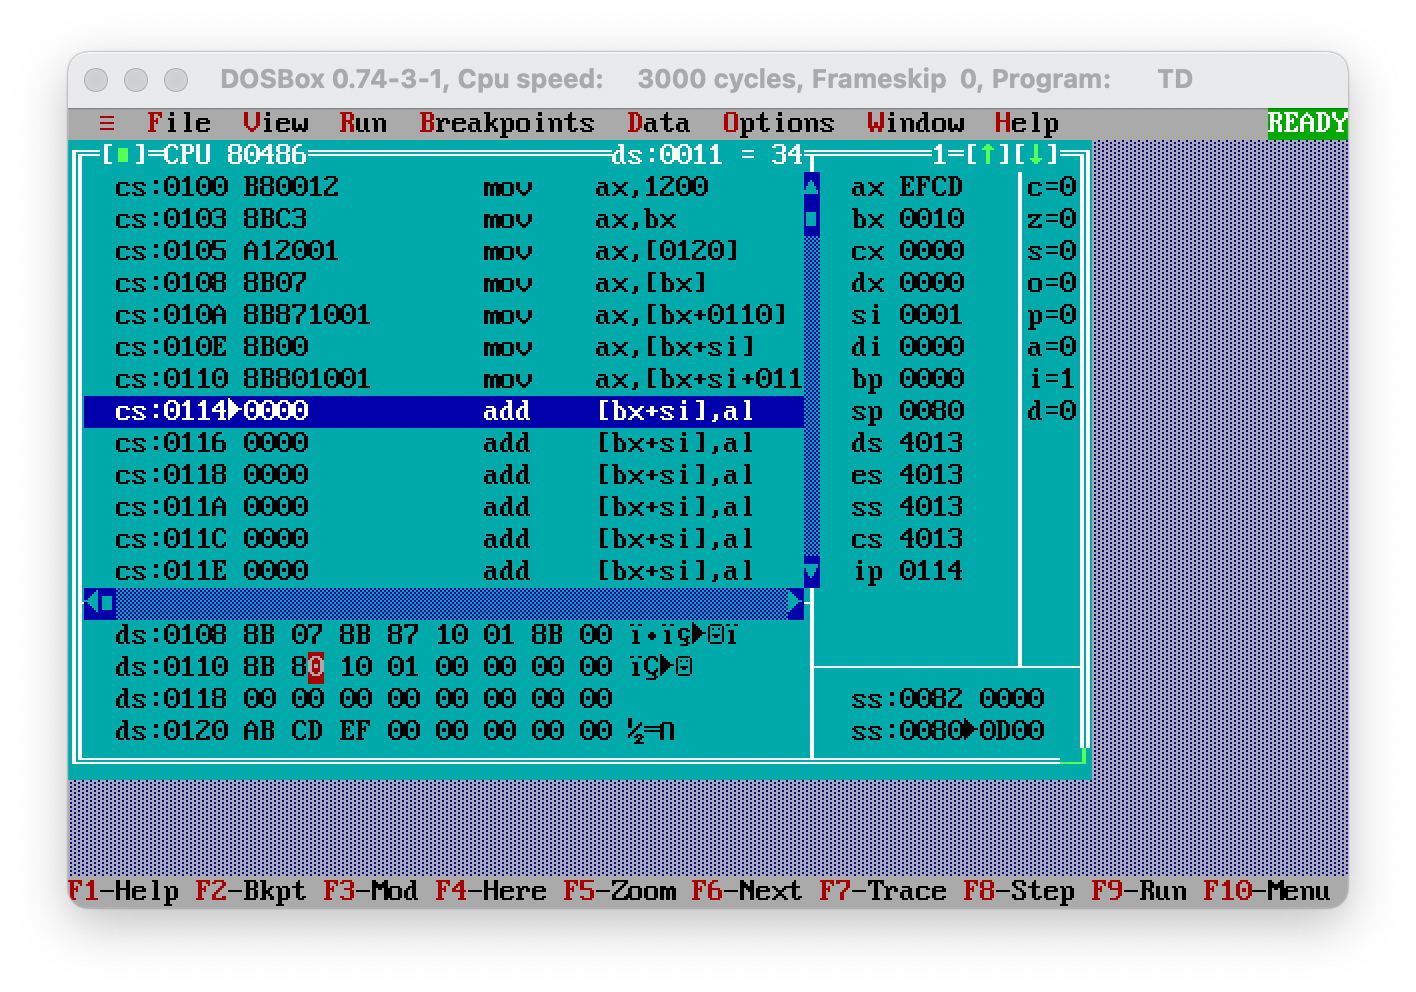
\includegraphics[width=0.7\textwidth]{fig/task4.png}
    \caption{实验四界面}
    \label{fig:task4} 
\end{figure}

\subsection{不同寻址方式传递数据}
实验前先检查寄存器情况:\texttt{DS=4013H, BX=0000H, SI=0000H};初始化数据段情况:\texttt{DS:[1000H]=FF, DS:[2020H]=00}。传递数据的代码段如下:
\begin{lstlisting}[language={[x86masm]Assembler},title=code]
    % 直接寻址
    MOV AL,[1000H]
    MOV [2020H],AL
    % 基址寻址
    MOV AH,1000[BX]
    MOV [2020H],AH
    % 变址寻址
    MOV AH,0100[SI]
    MOV [2020H],AH
\end{lstlisting}
经过上机验证,全部正确。
\begin{note}{语法错误}{}
    输入指令\texttt{MOV [2020H],[0100H]}会出现\texttt{"Syntax error"},原因是\texttt{MOV}指令的源、目标操作数不能同时为储存器,需要借助寄存器间接传递。
\end{note}

\subsection{数据的交换}
设\texttt{AX}寄存器中的内容为\texttt{1111H},\texttt{BX}寄存器中的内容为\texttt{2222H},\texttt{DS:0010H}单元中的内容为\texttt{3333H}。将\texttt{AX}和\texttt{BX}寄存器中内容进行交换,然后再将\texttt{BX}寄存器中的内容和\texttt{DS:0010H}单元中的内容进行交换。
\begin{lstlisting}[language={[x86masm]Assembler},title=code]
    % AX与BX交换
    XOR AX,BX
    XOR BX,AX
    XOR AX,BX
    % BX与储存器交换
    MOV CX,BX
    MOV BX,[0100H]
    MOV [0100H],CX
\end{lstlisting}
\begin{analyze}{数据交换方式}{}
    数据交换有多种方法:
    \begin{enumerate}
        \item 经典使用变量来进行交换;
        \item 通过三次异或来交换;
        \begin{idea}{异或特点}{}
            \begin{enumerate}
                \item 优点:\\节省变量成本;
                \item 缺点:\\会增加读写次数,使得程序运行时间较长;\\会影响标志位。
            \end{enumerate}
        \end{idea}
        \item 直接使用指令\texttt{XCHG}来交换数据,需要注意其中一个操作数必须在寄存器中!
        \item 可以利用命令\texttt{PUSH, POP}来进行交换,但需要将两个数据放在相邻的字节中(原因:两指令只能是字操作)。
        \item 除此之外还可以利用一些花哨的方法交换数据,但没意义。所谓“技巧”,只会让程序运行的更慢!
    \end{enumerate}
\end{analyze}

\subsection{传送数据段}
设\texttt{DS=1000H},\texttt{ES=2000H},有关存储器的内容见要求,将\texttt{DS}段的内容传送到\texttt{AX}寄存器;\texttt{ES}段的内容传送到\texttt{BX}寄存器,编写程序段。

代码指令如下
\begin{lstlisting}[language={[x86masm]Assembler},title=code]
    MOV WORD PTR AX,[0010]
    MOV WORD PTR BX,ES:[0020]
\end{lstlisting}

实验结果见图 \ref{fig:rlt7}。
\begin{figure}[htbp]
    \centering
    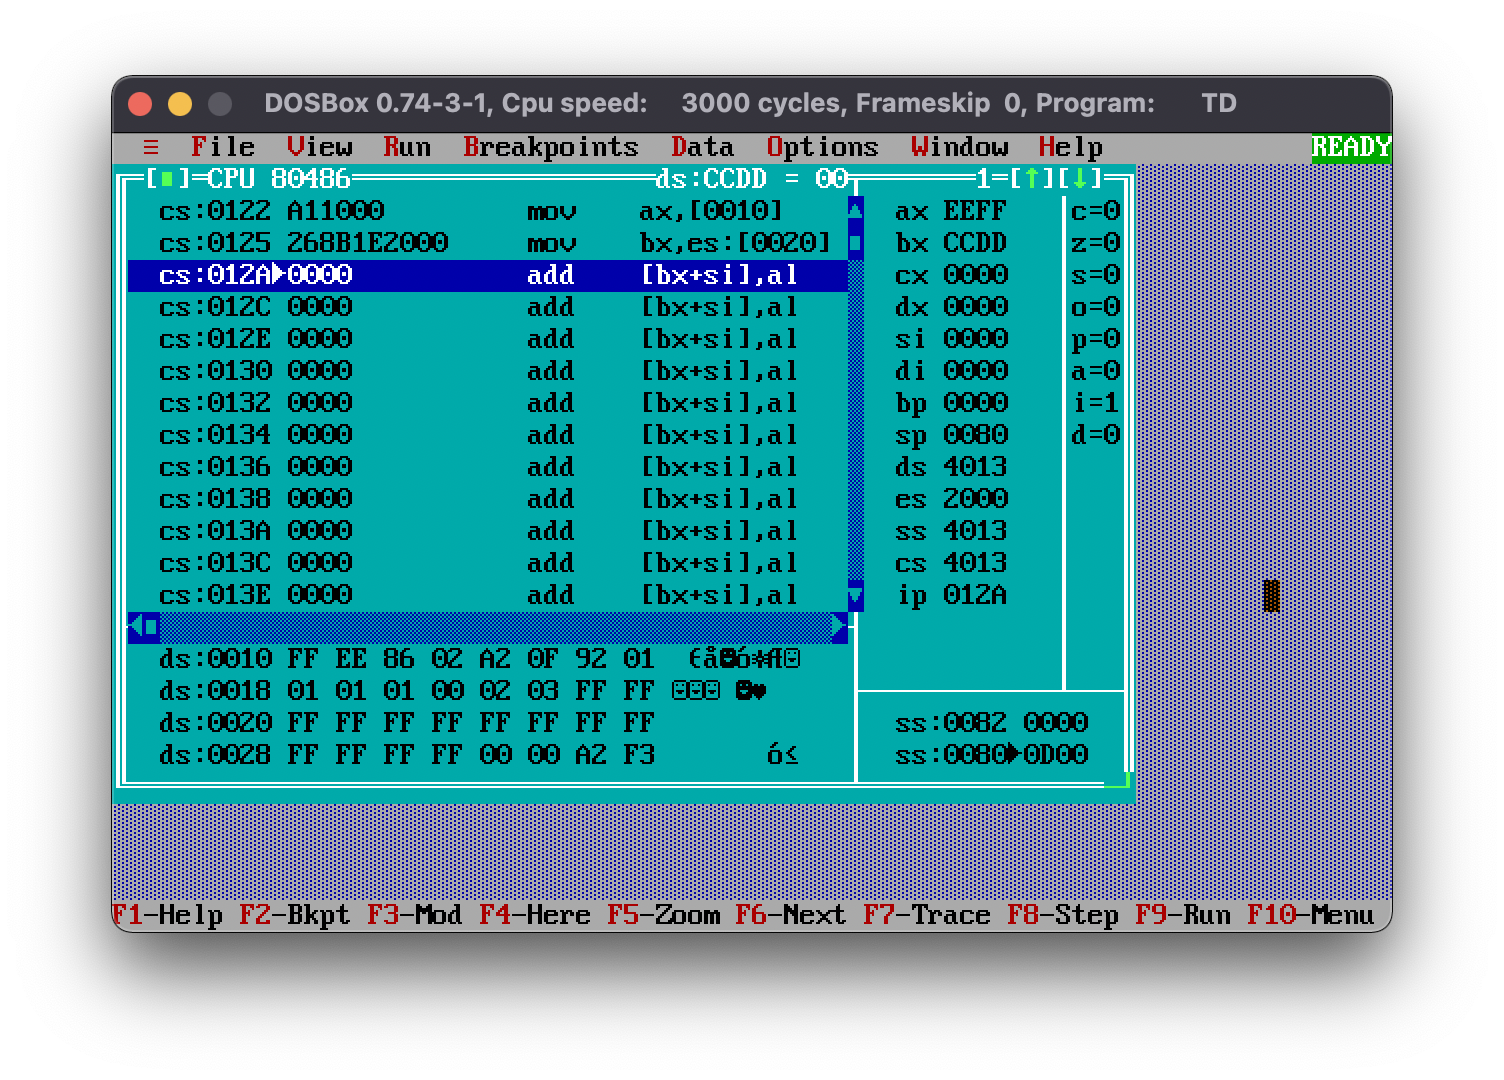
\includegraphics[width=0.7\textwidth]{fig/rlt7.png}
    \caption{实验结果}
    \label{fig:rlt7}
\end{figure}

\section{\texttt{TD}使用方法小结}
本课程实验中所需的\texttt{DOSBox}等软件搭建于\texttt{Mac OS}系统中,基本操作以及快捷键与\texttt{Windows}大致相同,不再赘述。全部文件已上传至我的\texttt{GitHub}主页 \cite{mygit}。

以下是符合个人喜好的个性化操作:
\begin{enumerate}
    \item \texttt{Mac OS}系统下的文件路径较于\texttt{Windows}系统较为复杂,因为实验前的自动挂载十分重要。具体方法为:通过\texttt{shift+cmd+.}找到根目录下\texttt{/Library/Preferences/DOSBox 0.74-3-1 Preferences}的默认文件,在文件最后插入如下代码即可完成自动挂载:
    \begin{lstlisting}[language={[x86masm]Assembler},title=code]
    mount c ~/DOSBox (your path) 
    path = path; c:\masm5
    c:
    \end{lstlisting}
    \item 实验报告采用 \LaTeX 模板进行编写,快捷键的设置也十分重要。在\texttt{vscode}中,使用组合键\texttt{fn+F1}搜索\texttt{keybingdings.json},进入可以添加快捷键,极大的提高了实验报告撰写效率。
    \item 关于实验报告,所有的目录、引用以及交叉引用全部赋予\texttt{Hyperlink},方便快速定位查找,提高了回溯报告的效率。
\end{enumerate}

\section{实验总结}
实验总结已随文附在“注意”、“思考”、“分析”中。

% 打印参考文献
\addcontentsline{toc}{section}{参考文献}
\printbibliography

\end{document}










%%%%%%%%%%%%%%%%%%%%%%%%%%%%%%%%%%%%%%%%%%%%%%%%%%%%%%%%

% 序号段落样例
\begin{enumerate}
    \item    
\end{enumerate}

% 表格样例
\begin{table}[htbp]
    \centering
    \caption{题目 \label{tab:parameters}}
    \bgroup\def\arraystretch{1.5}
    \setlength{\tabcolsep}{4.5mm}
      \begin{threeparttable}%要写注释,得加这行
        \begin{tabular}{c|c}
          \toprule
          \textbf{11} & \textbf{22}\\
          \midrule\midrule
          \grayrow  & \\
           & \\
          \grayrow  & \\ 
          \bottomrule
        \end{tabular}

        %注释
        \begin{tablenotes}%注释开始
        \footnotesize
        \item[$\ast$] $\mathtt{rand}\ [a, b]\ (a<b)$ is a random value generated between $a$ and $b$.
        \end{tablenotes}%注释结束
      \end{threeparttable}%要写注释,得加这行

    \egroup
\end{table}

% 插入图片样例
\begin{figure}[htbp]
    \centering
    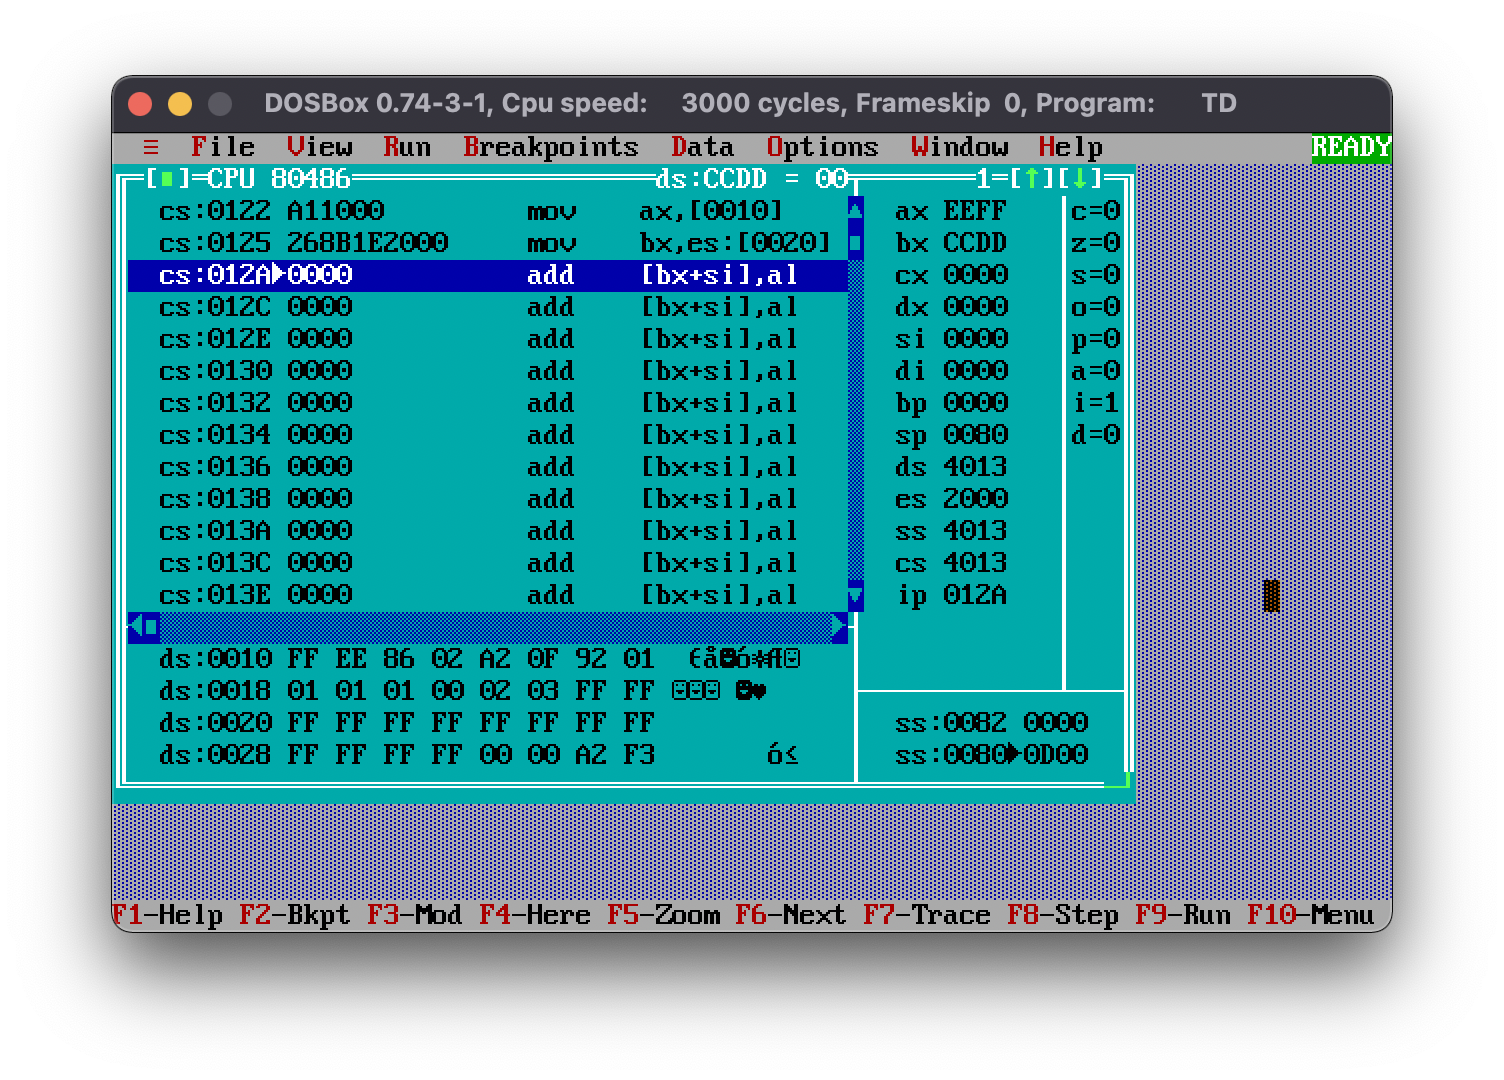
\includegraphics[width=0.7\textwidth]{fig/rlt7.png}
    \caption{}
    \label{fig:xxx}
\end{figure}

% 并排两张图样例
\begin{figure}[htbp]
    \centering
    \subfloat[原理图]{
        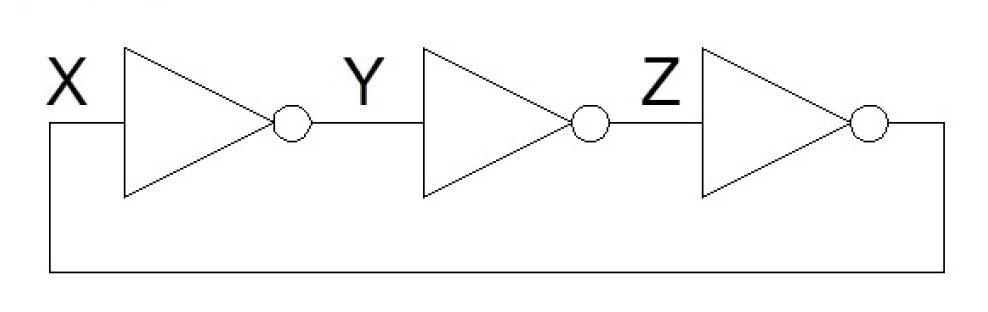
\includegraphics[height=2cm]{fig/oscillation_init.png}
        \label{subfig:oscillation_init}
    }
    \subfloat[等效图]{
        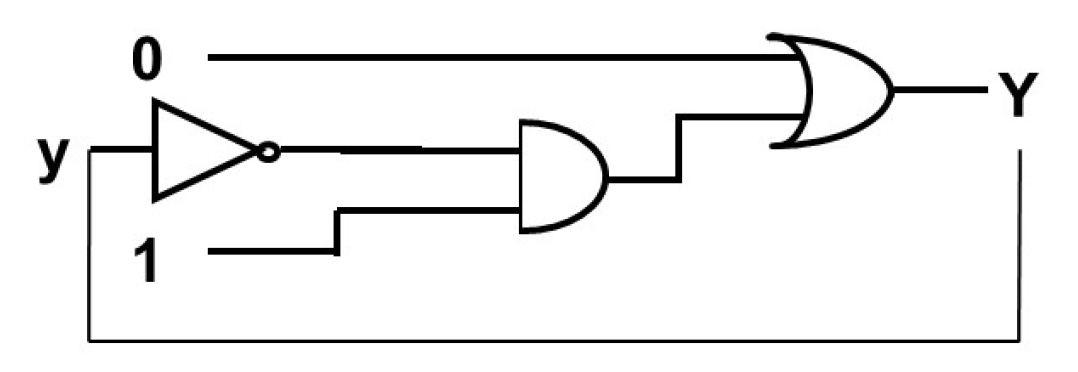
\includegraphics[height=2cm]{fig/oscillation_real.png}
        \label{subfig:oscillation_real}
    }
    \caption{}
    \label{fig:oscillation_circuit}
\end{figure}

% 注意样例(idea/analyze 分别表示思考和分析)
\begin{note}{题目}{}
    内容
\end{note}

% 代码样例
\begin{lstlisting}[language={[x86masm]Assembler},title=code]
    mycode
\end{lstlisting}